\documentclass[a4paper]{article}

\usepackage[portuguese]{babel}
\usepackage[utf8]{inputenc}
\usepackage{graphicx,hyperref}
\usepackage{float}
\usepackage{listings}
\usepackage{proof,tikz}
\usepackage{amssymb,amsthm,stmaryrd, amsmath}


\usepackage[edges]{forest}
\usetikzlibrary{automata, positioning, arrows}


\newtheorem{Lemma}{Lema}
\newtheorem{Theorem}{Teorema}
\theoremstyle{definition}
\newtheorem{Example}{Exemplo}
\newtheorem{Definition}{Definição}


\usepackage{fancyhdr}
  \pagestyle{fancy}
  \fancyhf{}
  \lhead{Teoria da Computação}
  \rhead{Aula 16}
  \lfoot{Prof. Rodrigo Ribeiro}
  \rfoot{\thepage}
  \renewcommand{\footrulewidth}{0.4pt}
  \pagestyle{fancy}

\tikzset{
        -,  % makes the edges directed
        >=stealth', % makes the arrow heads bold
        node distance=3cm,
        every state/.style={thick, fill=gray!10},
        initial text=$\,$
        }
  

\begin{document}

  \title{Aula 16 - Lema do bombeamento para linguagens livres de contexto}
  \author{Rodrigo Ribeiro}

  \maketitle


  \pagestyle{fancy}


  \section*{Objetivos}

  \begin{itemize}
     \item Apresentar e provar o lema do bombeamento para linguagens livres de contexto.
     \item Exemplos de uso do lema para mostrar que uma linguagem não é livre de contexto.   
  \end{itemize}

  \section{O lema do bombeamento}

  \begin{Lemma}
    Seja $L$ uma linguagem livre de contexto. Então, existe uma constante $k >
    0$ tal que para qualquer  palavra $z \in L$ com $|z| \geq k$ existem
    $u,v,w,x,y \in \Sigma^*$ que satisfazem as seguintes condições:
    \begin{itemize}
      \item $z = uvwxy$
      \item $|vwx| \leq k$
      \item $vx \neq \lambda$
      \item $forall i. i \geq 0 \to uv^iwx^iy \in L$
    \end{itemize}
  \end{Lemma}

  \begin{proof}
    Suponha $G = (V,\Sigma,R,P)$ uma GLC na FNC. Seja $k = 2^{|V| + 1}$.
    Suponha $z \in L(G)$ e que $|z| \geq k$. Como toda AD de uma GLC na FNC é
    binária, temos que a AD para $z$ tem altura não inferior a $|V| + 1$.
    Considere o maior caminho da raiz a uma das folhas nesta AD. Pelo princípio
    da casa dos pombos, algum terminal ocorre mais de uma vez neste caminho.
    Escolha a variável que repete pela primeira vez neste caminho iniciando das
    folhas para a raiz. A partir do formato da árvore de derivação (apresentado
    na figura a seguir) temos que $z = uvwxy$. 
    \begin{figure}[H]
      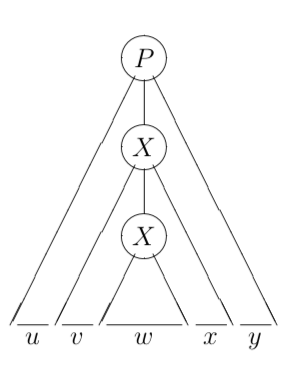
\includegraphics[scale=.4]{tree.png}
      \centering
    \end{figure}
    Como selecionamos a variável $X$
    a como sendo a primeira que repete no maior caminho iniciando das folhas
    para a raiz, temos que $|vwx| \leq n + 1 = k$. Uma vez que $G$ está na FNC,
    não pode ser o caso de $vx = \lambda$ pois, nesta situação, teríamos que a
    variável $X$ seria encadeada, o que não ocorre na FNC.  Evidentemente,
    podemos repetir derivações iniciando com $X$ um número $i\geq 0$, produzindo
    $ uv^iwx^iy \in L$.
  \end{proof}


  \begin{Example}
    Vamos usar o lema do bombeamento para mostrar que a linguagem
    $\{0^n1^n2^n\,|\,n\geq 0\}$ não é livre de contexto. A estratégia é similar
    ao lema do bombeamento para linguagens regulares.

    Suponha que $L = \{0^n1^n2^n\,|\,n\geq 0\}$ é uma LLC e seja $k$ a
    constante referida no lema. Seja $z = 0^k1^k2^k$. Como $|z|\geq k$, pelo LB
    as seguintes condições devem ser verdadeiras:
    \begin{itemize}
      \item $z = uvwxy$
      \item $|vwx| \leq k$
      \item $vx \neq \lambda$
      \item $forall i. i \geq 0 \to uv^iwx^iy \in L$
    \end{itemize}
    Suponha que $0^k1^k2^k = uvwxy$, $|vwx| \leq k$ e que $vx \neq \lambda$.
    Considere os seguintes casos:
    \begin{itemize}
      \item $vx$ contém algum $0$. Nessa situação, temos que $vx$ não possui
        nenhum $2$. Seja $ i= 0$. Temos que $uv^0wx^0y \not\in L$ pois terá
        menos 0's que 1's ou 2's.
      \item $vx$ não contém $0$. Nesse caso, $vx$ possui apenas 1's e 2's. Seja
        $i = 0$. Temos que $uv^0wx^0y \not\in L$ pois terá
        mais 0's que 1's ou 2's.
      \end{itemize}
      Logo, em ambos os casos, $uv^0wx^0y \not\in L$, contrariando o LB.
      Portanto, $L = \{0^n1^n2^n\,|\,n\geq 0\}$ não pode ser uma LLC.
  \end{Example}
  
  \section{Exercícios} 

  \begin{enumerate}
     \item Construa uma gramática equivalente na FNC.
       \[
         \begin{array}{l}
           P \to BPA \,|\,A \\
           A \to aA \,|\, \lambda\\
           B \to Bba \,|\,\lambda\\
         \end{array}
       \]
     \item Construa uma gramática equivalente na FNG
       \[
         \begin{array}{l}
           P \to A \,|\,BC\\
           A \to B \,|\, C\\
           C \to cC \,|\, c\\
         \end{array}
       \]
     \item Construa uma gramática equivalente na FNC.
       O alfabeto para essa gramática é $\{0,1,2\}$.
       \[
         \begin{array}{l}
           T \to 0\, |\, 1 \,|\, T\,T\,|\,2\,1\,T 
         \end{array}
       \]
     \item Mostre como construir uma gramática na FNC a partir de uma gramática
       na FNG.
  \end{enumerate}
\end{document}
